\chapter{Introduction}
\section{Motivation}
As a human being, we visually perceive and experience our whole world in terms of colors, resulting from various kinds of physical light interaction phenomenons. Particularly in biology, there are basically two main causes for color production. Firstly, due to pigmentation, which occures since certain molecules in a biological structure selectively absorb or reflect specific wavelengths from an incident light source. And secondly because of structural colors which are the result of physical interaction of light with a nanostructure, exclusively relying on the structring of the material and not any other property. One particular example for such biological color production are the colors we can see when having a closer look at the illuminated skin of snake species, as shown in figure $\ref{fig:snakespecies}$.

\begin{figure}[H]
  \centering
  \subfigure[Xenopeltis snake]{
    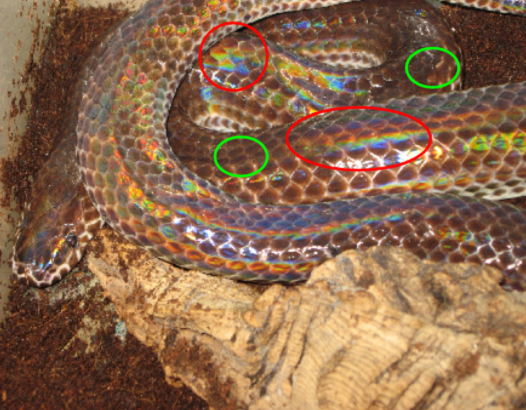
\includegraphics[scale=0.39]{background/xenopeltissnake.png}
    \label{fig:xenospeicies}
  }
~
  \subfigure[Elaphe Guttata snake]{
    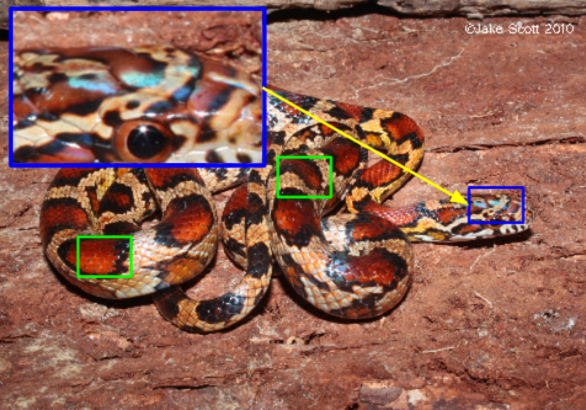
\includegraphics[scale=0.39]{background/elaphesnake.png}
    \label{fig:elpahespecies}
  }
  \caption[example biological color production]{Examples of pigmentation color (green circles) and structural color (red circles) on snake species$\footnotemark$.}
  \label{fig:snakespecies}
\end{figure}
\footnotetext{image source of figure $\ref{fig:xenospeicies}$ \texttt{http://www.snakes-alive.co.uk/gallery\textunderscore5.html} and figure $\ref{fig:elpahespecies}$ \texttt{http://www.the-livingrainforest.co.uk/living/view\textunderscore price.php?id=464}} 

Comparing both snake species with each other, we observe that the Xenopeltis species expresses structural colors in form of iridescent patterns along its scales way stronger than the Elaphe species does. The reason for this lies on the nanostructure of their skins. A natural diffraction grating is a semitransparent layer of biological nanostructures which exhibits a certain degree of regularity to produce structural colors by diffracting an incident light source. There are a vast amount of additional reasons for producing structural colors in nature, such as thin film interference, intra-cellular photonic crystyls or diffraction gratings. More detailed examples are listed in figure $\ref{fig:structuralcolorexamples}$. 

\begin{figure}[H]
  \centering
  \subfigure[Thin Film Inteference soapbubble]{
    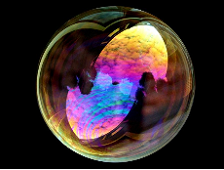
\includegraphics[scale=0.6]{background/soapbubble.png}
    \label{fig:soapbubble}
  }
~
  \subfigure[Multilayer Interference on abdomen of beetle]{
    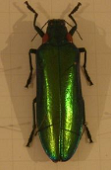
\includegraphics[scale=0.6]{background/beetle.png}
    \label{fig:beetle}
  }
~
  \subfigure[Photonic crystals in Wings of buttefly]{
    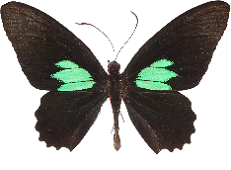
\includegraphics[scale=0.6]{background/butterflypc.png}
    \label{fig:butterflyphotoniccristals}
  }

  \subfigure[Scattering of light on butterfly wing]{
    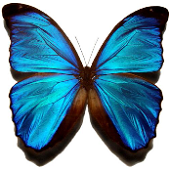
\includegraphics[scale=0.6]{background/butterflyscattering.png}
    \label{fig:butterflyscattering}
  }
~
  \subfigure[Artifical Diffraction Grating on CD]{
    
\includegraphics[scale=0.6]{background/cd.png}
    \label{fig:cddiffractiongrating}
  } 
~
  \subfigure[Natural Diffraction Grating on snake skin]{
    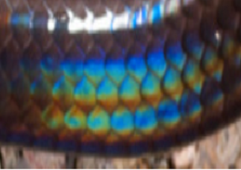
\includegraphics[scale=0.6]{background/snakeskin.png}
    \label{fig:snakediffractiongrating}
  }   
  
  \caption[Structural color examples]{Examples$\footnotemark$ for structural colors on the wings and the abdomen of insects, liquids, synthetic structures, and on scales on the skin of reptiles.}
  \label{fig:structuralcolorexamples}
\end{figure}
\footnotetext{image source of figure:
\begin{itemize}
  \item \ref{fig:soapbubble}: \texttt{http://www.ualberta.ca/\textasciitilde pogosyan/teaching/PHYS\textunderscore 130/FALL\textunderscore 2010/lectures/lect33/lecture33.html}
  \item \ref{fig:beetle}: \texttt{http://www.itp.uni-hannover.de/\textasciitilde zawischa/ITP/multibeam.html}
  \item \ref{fig:butterflyphotoniccristals}: \texttt{http://upload.wikimedia.org/wikipedia/commons/a/a4/Parides\textunderscore sesostris\textunderscore MHNT\textunderscore dos.jpg}
  \item \ref{fig:butterflyscattering}: From paper \cite{struccolor}, figure 6.
  \item \ref{fig:cddiffractiongrating}: \texttt{http://cnx.org/content/m42496/latest/?collection=col11428/latest}
  \item \ref{fig:snakediffractiongrating}: \texttt{http://www.snakes-alive.co.uk/gallery\textunderscore 5.html}
  \end{itemize}
}

Already in the 17th century Robert Hooke was able to relate the cause of structural colors to the the microstructure of a material. During his examinations of peacock feathers he found that the colors could be made disappear by wetting the feathers and further observerd that the feathers are made of tiny ridges. Building on top of the latest knowledge about interference, Newton related structural colors with wave interference. Nowadays, in the field of computer graphics, many researchers have been attempted rendering structural colors but unforunately, most currently available approaches are not able to perfrom interactive rendering or are oversimplified and thus cannot model accurately the effect of diffraction.

\section{Goals}
The purpose of this thesis is to simulate realistically by rendering structural colors caused by the effect of diffraction on different biological structures in realtime. We focus on structural colors generated by diffraction gratings, in particular our approach applies to surfaces with quasiperiodic structures at the nanometer scale that can be represented as heighfields. such structures are found on the sehds of snkaes, wings of butterflies or the bodies of various insects. we restrict ourself and focus on different snake skins sheds which are acquired nanoscaled heightfields using atomic force microscopy. 

In oder to achieve our rendering purpose we will rely J. Stam's formulation of a BRDF which basically describes the effect of diffraction on a given surface assuming one knows the hightfield of this surface and will further extend this. Appart from Stam's approach, which models the heightfield as a probabilistic superposition of bumps and proceeds to derive an analytical expression for the BRDF, our BRDF representation takes the heightfield from explicit measurement. 
I.E. in our case, those heightfields are small patches of the microstructured surfaces (in nano-scale) taken by AFM of snake skin patches provided by our collaborators in Geneva..
So this approach is closer to real truth, since we use measured surfaces instead of statistical surface profile.

Therefore, this work can be considered as an extension of J. Stam's derivations for the case one is provided by a explicit height field on a quasiperiodic structure.

Real time performance is achieved with a representation of the formula as a power series over a variable related to the viewing and lighting directions. Values closely related to the coefficients in that power series are precomputed.

The contribution is that this approach is more broadly applicable than the previous work. Although the previously published formula theoretically has this much flexibility already, there is a novel contribution in demonstrating how such generality can be leveraged in practical implementation


\section{Previous work}
stam, hooke, see our paper, see stams paper, see own research.


Robert Hooke = observed connection between microscopic structures and colorisation
wave nature of light led to conclusion that the cause for the coloration lies in wave interference.

previous

In computer graphics literature, Stam was the first to develop reflection models based on wave optics called diffraction shaders, that can produce colorful diffraction effects. His approach is based on a far field approximation of the Kirchhof integral. He shows that for surfaces representeted as nanoscale heightfieds it is possible to derive their BRDF as the Fourier transformation of a function of the heightfield. Nevetheless, this formulation is not immediately useful for efficent rendering of measured complex nanostructures since this would require the on-the-fly evaluation of and and integration over Fourier transforms of the heightfield that depend on the light and viewing geometry. In his derivations, Stam models heightfields as probabilistic superpositions of bumps forming periodic like structures. This provides him an analytical identity for this class of heightfields. However, boplogocal nanostructures are way more complex and do not lend themself to this simplified statistical model.

follow ups


\section{Overview}
The reminder of this thesis is organized as the follows: due to the fact that this thesis has a rather advanced mathematical complexity the first part of chapter 2 introduces some important definitions which are required in order to be able to follow the derivations in the last third of chapter 2. Before starting the derivations, a brief summary of J. Stam's Paper about diffraction shaders is provided since this whole thesis is based on his BRDF representation. Our derivations itself are listed step-wiese, whereas there is a final representation provided by the end of chapter 2. Chapter 3 addresses the practical part of this thesis, the implementation of our diffraction model, explaining all precomputation steps and how rendering is preformed in our developed framework for this thesis. Chapter 4  gives some further insight about diffraction by explaining the topic about diffraction grating in depth. Furthermore, within this chapter we evaluates the qualitative validity of our BRDF models applied on different surface gratings by computing their reflectance and comparing this to the grating equation under similar conditions. Chapter 5 presents our rendered results, first the so called BRDF maps for all our gratings and shading approaches under various shading parameters and then the actual renderings on a snake mesh. Chapter 6 contains the conclusion of this thesis which starts by a review briefly discussing what has been achieved in this thesis and the drawbacks. There are also some words about my personal experience during this thesis.
